\section{常见ORAM体制研究进展}
\subsection{ORAM常用的技术}
\subsubsection{不经意排序}
\textit{不经意排序 (Oblivious sort)},又称为茫然排序,是指这样一种排序算法,其排序过程对数据操作的顺序是\textit{预定义、固定的},如冒泡排序是典型的茫然排序,而选择排序则不是 (顺序依赖于数据中每一轮的最大值) 。时间复杂性较好的茫然排序有$O(n\log^2{n})$的Batcher排序网络和$O(n\log{n})$的AKS排序网络,然而后者的常数项 ($\approx{6100}$) 远大于前者 ($\approx{0.5}$) ,因此实用中通常采用理论复杂度更高的前者。
\subsubsection{不经意随机排列}
\textit{不经意随机排列 (Oblivious random permutation)},在许多ORAM体制对数据的预处理与混洗 (shuffle) 中用到。我们通常采用Knuth洗牌算法:
\begin{algorithm}[H]
    \label{alg:Knuth}
    \caption{Knuth shuffle algorithm}
    \begin{algorithmic}[1]
        \Procedure {shuffle}{$A,N$}
            \For{$i \gets 0 \ \mathbf{to}\ N-1$}
                \State $j \gets random(0,N-1)$
                \State \Call{swap}{$A_i,A_j$}
            \EndFor
		\EndProcedure
    \end{algorithmic}
\end{algorithm}

\subsection{平方根模型}
\textit{Square Root ORAM}是第一个在文献中提出的ORAM模型\cite{ref5},分为\textit{Basic Square Root ORAM (Basic-SR)}及其改进\textit{Interleave Buffer Shuffle Square Root ORAM (IBS-SR)}。
\subsubsection{Basic-SR}
在这个ORAM中,服务器的结构如下:服务器共储存$N+2\sqrt{N}$个数据块,其中$N$个为加密过的真实数据块,$\sqrt{N}$个为用于混淆的伪数据块(dummy block),最后$N$个为缓冲区(shelter)。\par
\noindent Basic-SR的算法流程如下:
\begin{enumerate}
    \item 对前$N+\sqrt N$个数据块,也就是真实数据块与伪数据块一起进行随机排列。
    \item 扫描缓冲区$\sqrt N$个数据块
    \begin{itemize}
        \item $j$在缓冲区中,则对缓冲区进行一次伪数据块读写
        \item $j$不在缓冲区中,则从$j$的位置$\pi(id_j)$中读取数据并写入伪数据块
    \end{itemize}
    \item 进行第二次缓冲区扫描,如果是写操作就在缓冲区中更新数据,读操作就写入伪数据块。
    \item 当计数器$count$增加到$\sqrt N$时,就要对所有数据块进行不经意排序,否则访问模式就会有泄漏的风险。
\end{enumerate}
伪代码如下:
\begin{algorithm}[H]
    \label{alg:BSR}
    \caption{Basic-SR ORAM}
    \begin{algorithmic}[1]
        \State $p \gets 0$
        \While{\textbf{true}}
            \State $p \gets p+1$
            \State Perform an oblivious random permutation $\pi$ of the blocks in the first $(N + \sqrt N)$ locations (data + dummy blocks)
            \For{$count \gets 1\ \mathbf{to}\ \sqrt N$}
                \State $j\gets (p-1)\sqrt N+count$
                \If{$id_j$ in shelter location $x\ (N+\sqrt N+1\leq x\leq N+2\sqrt N)$}
                    \State Read a dummy block from $\pi(N+count)$
                    \State Write back this dummy block
                \Else\Comment{$id_j$ not in shelter}
                    \State $x\gets -1$, read $id_j$ from $\pi(id_j)$
                    \State Write a dummy block to $\pi(id_j)$
                \EndIf
                \For{$i\ \gets 1\ \mathbf{to}\ \sqrt N$}\Comment{scan the shelter}
                    \State Read shelter block $N+\sqrt N+i$
                    \If{$N+\sqrt N+i=x$}
                        \If{$op_j=write$}
                            \State Write $block_j$ to $N+\sqrt N+i$
                        \Else\Comment{$op_j=read$}
                            \State Write the same data back to $N+\sqrt N+i$
                        \EndIf
                    \ElsIf{$i=count \and x=-1$}
                        \If{$op_j=write$}
                            \State Write $block_j$ to $N+\sqrt N+i$
                        \Else\Comment{$op_j=read$}
                            \State Write the same data back to $N+\sqrt N+i$
                        \EndIf
                    \Else
                        \State Write a dummy block to $N+\sqrt N+i=x$
                    \EndIf
                \EndFor
            \EndFor
            \State Perform an oblivious sort on all $(N + 2\sqrt N)$ locations
        \EndWhile
    \end{algorithmic}
\end{algorithm}
平方根模型以$\sqrt N$次访问为一轮。在每一轮访问中,保证前面每个数据块的位置只会被访问一次,之后被访问的数据块就会被载入缓冲区shelter中。而对缓冲区shelter的查找与访问都会扫描整个缓冲区,以保证不会泄露访问模式。每一轮访问结束之后,所有数据就要重新排序混洗。\par
Basic-SR ORAM模型,对每一轮访问($\sqrt N$次),摊还时间复杂度由不经意排序的复杂度决定,为$O(\sqrt N\log^2 N)$(Batcher排序网络)或$O(\sqrt N\log N)$(AKS排序网络)。
\subsubsection{IBS-SR}
IBS-SR是对平方根模型的一个简要改进\cite{ref6},服务器储存$N$个数据块和$\sqrt N$个伪数据块,而对客户端有$O(\sqrt N)$的内存空间复杂度。\par
IBS-SR的改进在于,使用哈希函数,每次对哈希映射到的$\sqrt{N+\sqrt{N}}$个数据块进行混洗并更换哈希映射,以代替Basic-SR中$O(N\log^2 N)$的不经意排序操作,该混洗操作称为\textit{Interleave Buffer Shuffle (IBS)}。从而突破了不经意排序的性能瓶颈,使得ORAM的摊还时间复杂度降为$O(\sqrt{N})$。

\subsection{层次模型}
\textit{Hierarchical ORAM}是文献\cite{ref5}中提出的另一种ORAM,相比Square Root ORAM,Hierarchical ORAM的效率比较高。\par
\textit{Basic Hierarchical ORAM (Basic-HR)}将服务器存储空间划分为$L=\lceil\log_2N\rceil$层,每层$\ell (1\leq\ell\leq L)$中有$2^\ell$个桶,则每层的桶的个数恰好是上一层中的两倍。每$2^\ell$次操作后,第$\ell$层就会被混洗。初始化的时候,要为每一层选择一个hash函数,用于决定数据块应放入哪个桶中。
\begin{figure}[H]
    \centering
    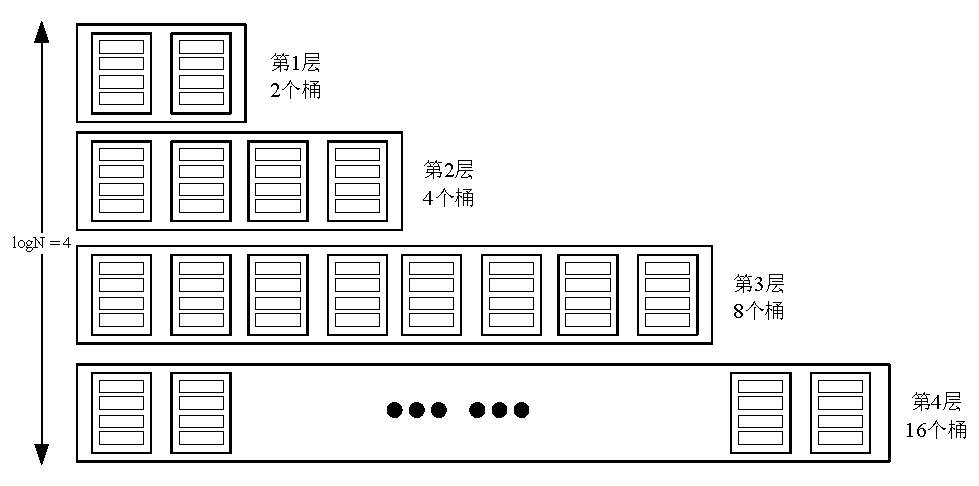
\includegraphics[width=0.8\textwidth]{orams/hierarchical.pdf}
    \caption{$L=4$时Hierarchical ORAM的数据结构}
    \label{fig:hier}
\end{figure}
Basic-HR算法流程如下:
\begin{enumerate}
    \item 从第1层到第L层,逐层根据哈希函数扫描数据块$id_j$可能在的桶。如果在之前的层中已经找到,则随机选一个桶来读写。如果在该层找到,则读取后写回一个伪数据块。如果没有找到,则读取并原样写回该桶的数据块。
    \item 所有层搜索完毕后,将数据块$id_j$写入第一层。
    \item 每进行$2^\ell$次操作,就要将$\ell$层与$\ell+1$层数据块混洗,并且哈希函数要重新选取。
\end{enumerate}
伪代码如下:
\begin{algorithm}[H]
    \label{alg:BHR}
    \caption{Basic-HR ORAM}
    \begin{algorithmic}[1]
        \State $j \gets 0$
        \While{\textbf{true}}
            \State $j \gets j+1$
            \For{$\ell \gets 1\ \mathbf{to}\ L$}
                \If{block $id_j$ hasn't been found}
                    \State Scan hash bucket to find $id_j$
                    \If{$id_j$ found}
                        \State Write a dummy block back
                    \Else
                        \State Write the original block back
                    \EndIf
                \Else\Comment{$id_j$ has been found}
                    \State Read and write a random block in level $\ell$
                \EndIf
            \EndFor
            \If{$j$ is odd}
                \State Write block $id_j$ into 1st bucket in level 1.
            \Else
                \State Write block $id_j$ into 2nd bucket in level 1.
            \EndIf
            \State $d \gets \max\{1\leq x\leq L: j\bmod 2^x = 0\}$
            \For{$\ell \gets 1\ \mathbf{to}\ d$}\Comment{shuffle every $2^\ell$ operations}
                \State Pick a new hash function for level $\ell+1$
                \State Shuffle data in level $\ell$ and level $\ell+1$ using the new hash function.
            \EndFor
        \EndWhile
    \end{algorithmic}
\end{algorithm}
复杂度分析上,云端服务器的空间开销为$O(N\log N)$,客户端空间开销为$O(1)$。摊还时间复杂度由不经意排序的复杂度决定,为$O(\log^4 N)$(Batcher排序网络)或$O(\log^3 N)$(AKS排序网络)。与平方根模型相比有显著提升,但仍开销较大。

\subsection{分区模型}
\textit{TP-ORAM}是文献\cite{ref7}中提出的一种对层次模型的改进,其核心思想为将服务器分区(partition),将单个大小$N$分割为$\sqrt N$个小型ORAM,每个分区相当于一个ORAM的黑盒子,并不依赖具体的内部实现。\par
TP-ORAM中,分为$P=\sqrt{N}$个分区,每个分区采用层次模型,因此每个分区内有$L=\log_2{\sqrt{N}}+1=\frac{1}{2}\log_2N+1$层。与Basic-HR一样,第$\ell$层有$2^\ell$个块。为了防止随机误差导致的可能溢出,第$L$层有$2^L+\epsilon=2\sqrt{N}+\epsilon$个区块。通过简单的几何级数求和可以知道,每个分区一共有$4\sqrt{N}-2+\epsilon$个区块,而在具体实现\cite{ref7}中,被进一步放宽为$4.6\sqrt{N}$。除了分块内存,服务器中还存在$O(\sqrt{N})$大小的缓冲区(stash),stash被分为$P$块,每块对应服务器内存的一个分区。另外还有一个映射表(position map)来决定每一个数据块$id_j$被分配到哪个分区中。
\begin{figure}[H]
    \centering
    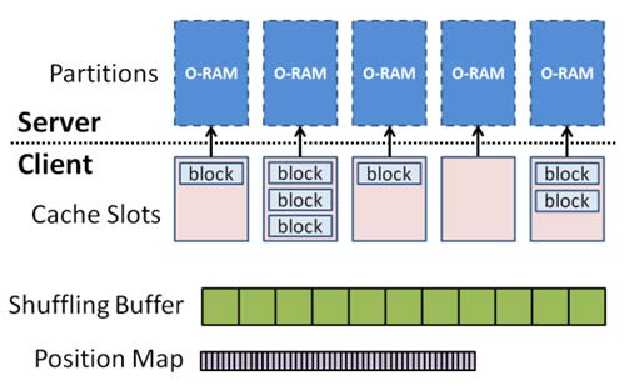
\includegraphics[width=0.8\textwidth]{orams/partition.pdf}
    \caption{分区模型的数据结构}
    \label{fig:part}
\end{figure}
\noindent TP-ORAM的主要流程如下:
\begin{enumerate}
    \item 通过映射表获取$id_j$所在的分区。先访问缓冲区,如果找到就读取出来并对内存分区进行一次伪访问;否则从内存分区中访问$id_j$。
    \item 随机选择另一个分区编号$r$,更新映射表并将$id_j$放到新的缓冲区中。
    \item 进行两次驱逐操作。
\end{enumerate}
伪代码如下:
\begin{algorithm}[H]
    \label{alg:TP}
    \caption{TP-ORAM}
    \begin{algorithmic}[1]
        \State $j \gets 0, s \gets 1$
        \While{\textbf{true}}
            \State $j \gets j+1$
            \State $p \gets position[id_j]$
            \If{block $id_j$ found in $stash[p]$}
                \State Read and delete $id_j$ from $stash[p]$
                \State Read a dummy block from partition $p$
            \Else\Comment{$id_j$ not in stash}
                \State Read $id_j$ from partition $p$
            \EndIf
            \State $r \gets random(1,P)$
            \State $position[id_j] \gets r$
            \State add $id_j$ into $stash[r]$
            \State\Call{Evict}{p} \Comment{Piggy-backed eviction}
            \State\Call{SequentialEvict}{$\nu$} or \Call{RandomEvict}{$\nu$}
        \EndWhile
    \end{algorithmic}
\end{algorithm}
驱逐操作(eviction)分为两个过程,第一个eviction过程是捎带式(Piggy-backed)的,也就是客户端执行一次访问之后,就会执行一次驱逐操作。驱逐操作将缓冲区中的一个元素“驱逐”回内存分区中,并对缓冲区写入一个伪数据。\par
第二步称为背景式(Background)驱逐,取决于一个频率参数$\nu$,每次数据访问之后,都会执行$\nu$次eviction操作。如果$\nu<1$说明多次访问之后才会执行一次背景式eviction操作。而背景式eviction操作有两种策略,一种是顺序驱逐,另一种是随机驱逐。
\begin{algorithm}[H]
    \caption{Evict}
    \begin{algorithmic}[1]
        \Procedure{Evict}{$p$}
            \If{$stash[p]$ is empty}
                \State Write a dummy block to partition $p$
            \Else
                \State Write a block from $stash[p]$ to partition $p$ and remove it from $stash[p]$
            \EndIf
        \EndProcedure
    \end{algorithmic}
\end{algorithm}
\begin{algorithm}[H]
    \caption{Sequential and Random Evict}
    \begin{minipage}{0.5\textwidth}
        \begin{algorithmic}[1]
            \Procedure{SequentialEvict}{$\nu$}
                \State $num \gets \mathcal{D}(\nu)$
                \Comment{$\mathcal{D}$ is a prescribed distribution}
                \For{$i \gets 1\ \mathbf{to}\ num$}
                    \State $count \gets count+1$
                    \State\Call{Evict}{$count$}
                \EndFor
            \EndProcedure
        \end{algorithmic}
    \end{minipage}
    \begin{minipage}{0.5\textwidth}
        \begin{algorithmic}[1]
            \Procedure{RandomEvict}{$\nu$}
                \State $num \gets \mathcal{D}(\nu)$
                \For{$i \gets 1\ \mathbf{to}\ num$}
                    \State $r \gets random(1,P)$
                    \State\Call{Evict}{$r$}
                \EndFor
            \EndProcedure
        \end{algorithmic}
    \end{minipage}
\end{algorithm}
复杂度分析上,云端服务器的空间开销为$O(N)$,客户端空间开销为$O(\sqrt{N}+\frac{N}{B})$,$O(\sqrt{N})$为缓冲区而$O(\frac{N}{B})$为映射表($B$为每个数据块的大小)。摊还时间复杂度可以低至$O(\log N)$,最坏情况为$O(\sqrt{N})$。分区模型相比于传统的模型而言有着显著的提升,但最坏情况依然开销较大。

\subsection{Basic Binary-Tree ORAM}
文献\cite{ref8}中提出了一种全新的树状模型,它不需要进行不经意排序和混洗操作,可以将ORAM操作的\textbf{最坏时间复杂度}控制在对数多项式以内,完成了一次显著的突破。\par
\textit{Basic Binary-Tree ORAM (BB-ORAM)}将整个服务器存储看做一棵平衡二叉树,而每个数据块映射到二叉树的每个叶节点。同时,客户端需要维护一个映射表(position map)来确定每个数据块所在的节点。

\subsection{Path-ORAM}
\textit{Path-ORAM}是文献\cite{ref9}中对BB-ORAM的一种改进,其思想同样采用树状模型,而在实现细节上有所优化。\par
与BB-ORAM一样,Path-ORAM把整个服务器存储看做一棵高为$L=\lfloor\log N\rfloor$的二叉树,树上的每个节点上有一个大小为$Z$的桶(bucket),其中含有真实数据块与伪数据块。每一个叶子节点$x\in\{0,1,\ldots,2^L-1\}$可以唯一确定一条从根到叶子的路径,令$\mathcal{P}(x)$为路径上所有桶的集合,特别地,$\mathcal{P}(x,\ell)$表示路径上第$\ell$层的桶。另外,客户端上有一块$O(\log N)$的缓冲区(stash),以及需要维护一块$O(\frac{N}{B})$的映射表。
\begin{figure}
    \centering
    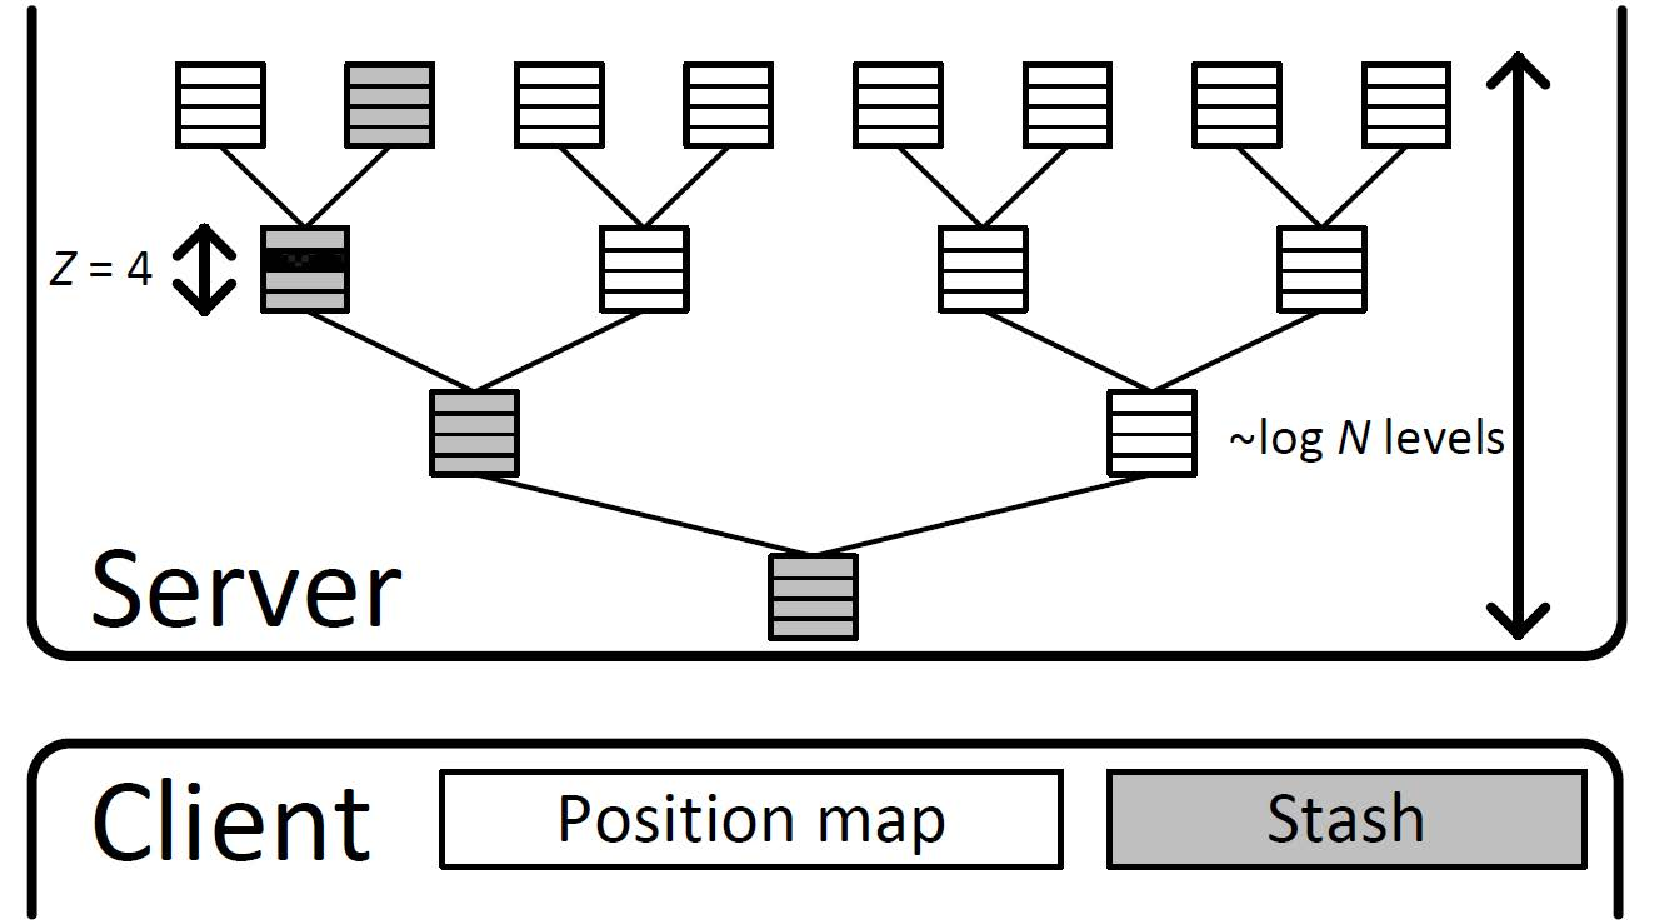
\includegraphics[width=0.65\textwidth]{orams/path.pdf}
    \caption{Path-ORAM的树状结构}
    \label{fig:path}
\end{figure}
\noindent Path-ORAM的算法流程如下:
\begin{enumerate}
    \item 通过映射表获取$id_j$所对应的叶节点$x$,并更新映射表,将$id_j$随机重新映射到另一个叶节点上。
    \item 将路径$\mathcal{P}(x)$上的所有桶全部读取到缓冲区中
    \item 如果是写操作,则写入$block_j$
    \item 将缓冲区中的数据尽可能写入回$\mathcal{P}(x)$中,其中一些本来不映射到$x$的数据也可能写入到第$\ell$层,只要$\mathcal{P}(x,\ell)=\mathcal{P}(x',\ell)$,即$x$路径与$x'$路径在第$\ell$层之前部分重合,那么该数据也可以写入到$\mathcal{P}(x,\ell)$中。
\end{enumerate}\par
这样,在服务端看来,客户端每次访问都是读取并写入一条随机的路径,因此访问模式不会被泄露。伪代码如下:
\begin{algorithm}[H]
    \label{alg:Path}
    \caption{Path-ORAM}
    \begin{algorithmic}[1]
        \State $j \gets 0, s \gets 1$
        \While{\textbf{true}}
            \State $j \gets j+1$
            \State $x \gets position[id_j]$
            \State $position[id_j] \gets random(0,2^L-1)$
            \For{$\ell \gets 0\ \mathbf{to}\ L$}
                \State $S \gets S \cup \mathcal{P}(x,\ell)$\Comment{$S$ denotes the stash}
            \EndFor
            \State data $\gets$ Read $id_j$ from $S$
            \If{$op_j=write$}
                \State $S \gets (S-\{(id_j,data)\})\cup\{(id_j,block_j)\}$\Comment{update old data to $block_j$}
            \EndIf
            \For{$\ell \gets L\ \mathbf{to}\ 0$}
                \State $S' \gets \{(a',data')\in S: \mathcal{P}(x,\ell)=\mathcal{P}(position[a'],\ell)\}$
                \Comment{$S'$ denotes the datas to write back in level $\ell$}
                \State $S' \gets$ Select $\min(|S'|,Z)$ from $S'$
                \State $S \gets S - S'$
                \State Write $S'$ into bucket $\mathcal{P}(x,\ell)$
            \EndFor
        \EndWhile
    \end{algorithmic}
\end{algorithm}
Path-ORAM原理简单,却极其高效,而二叉树的良好特性使其复杂度比之前的模型有了明显的提升。服务端空间需求为$O(N)$,而客户端的空间需求为$O(\log N+\frac{N}{B})$,即缓冲区加上映射表的大小。\par
时间复杂度方面,由于每次操作只需遍历一条路径,则平均与最坏时间复杂度都与树的高度成正比,即$O(\log N)$。带宽的消耗也优化到了对数级别,总带宽为$O(\frac{\log^2N}{\log B})$,平均带宽为$O(\frac{\log N}{\log B})$,只要$B=\Omega(\log^2N)$,Path-ORAM将比之前所有的ORAM模型拥有更低的复杂度\cite{ref9}。